%
% LaTeX report template 
%

% This is a comment: in LaTeX everything that in a line comes
% after a "%" symbol is treated as comment

\documentclass[11pt, a4paper]{article}
\usepackage{graphicx}
\usepackage{amsmath}
\usepackage{listings}
\usepackage{url}
\usepackage{float}
\usepackage{xcolor}

\definecolor{codegreen}{rgb}{0,0.6,0}
\definecolor{codegray}{rgb}{0.5,0.5,0.5}
\definecolor{codepurple}{rgb}{0.58,0,0.82}
\definecolor{backcolour}{rgb}{0.95,0.95,0.92}

\lstdefinestyle{mystyle}{
    backgroundcolor=\color{backcolour},   
    commentstyle=\color{codegreen},
    keywordstyle=\color{magenta},
    numberstyle=\tiny\color{codegray},
    stringstyle=\color{codepurple},
    basicstyle=\ttfamily\footnotesize,
    breakatwhitespace=false,         
    breaklines=true,                 
    captionpos=b,                    
    keepspaces=true,                 
    numbers=left,                    
    numbersep=5pt,                  
    showspaces=false,                
    showstringspaces=false,
    showtabs=false,                  
    tabsize=2
}

\lstset{style=mystyle}

\title{EE2703: Applied Programming Lab \\ Assignment No 8: The Digital Fourier Transform} % Title

\author{Ishaan Agarwal \\ EE20B046} % Author name

\date{\today} % Date for the report
\begin{document}		
		
\maketitle % Insert the title, author and date

\section{Introduction}
This assignment is based on calculation of the Discrete Fourier Transform (DFT) of signals. Fast Fourier Tansform (FFT) is an efficient implementation of DFT. For this, we use the numpy library which contains the \texttt{fft} module which can be used to calculate the fast fourier transform of a signal. In the last question we also try to approximate the CTFT of a gaussian by changing the window size and number of samples. 

\section{Questions}
\subsection{Question 1}
\subsubsection{Random data}
We find the Fourier Transform of a random signal and then we find the inverse Fourier Transform of the function, we then finally compare those values with the actual values generated,  we find that the max error we get is of the order of -16, thus our approximation is pretty good.

\begin{lstlisting}[language = Python]
#testing fft and ift
x = np.random.randn(100)
#dft
x_dft = np.fft.fft(x) 
#ift
x1 = np.fft.ifft(x_dft)
np.abs(x-x1).max()
\end{lstlisting}

\subsubsection{Spectrum of $\sin{5t}$}
Next we wanted to find the spectrum of $\sin{5t}$. We can write $\sin(5t)$ as:
$$\sin(5t) = 0.5(\frac{e^{5t}}{j}-\frac{e^{-5t}}{j})$$
So we can expect to get two peaks at +5 and -5 of height 0.5. The phase at the point of peaks is expected to be $\frac{\pi}{2}$ and $\frac{-\pi}{2}$ respectively based on the expansion of the sine wave.

\begin{lstlisting}[language = Python]
#plotting the spectrum of sin(5t)
x=linspace(0,2*pi,128)
y=sin(5*x)
Y=fft(y)

subplot(2,1,1)
plot(abs(Y),lw=2)
ylabel(r"$|Y|$",size=16)
title(r"Spectrum of $\sin(5t)$")
grid(True)
subplot(2,1,2)
plot(unwrap(angle(Y)),lw=2)
ylabel(r"Phase of $Y$",size=16)
xlabel(r"$k$",size=16)
grid(True)
show()
\end{lstlisting}

The following plot is obtained:
\begin{figure}[H]
     \centering
     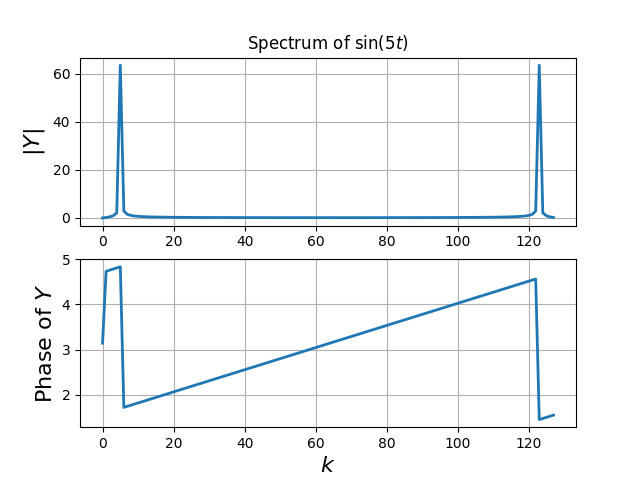
\includegraphics[scale=0.8]{Figure_1.png}
\end{figure}

We need to shift the phase plot so that it goes from $-\pi$ to $\pi$,  as 0 and $2\pi$ means the same thing. This can be done using the following code:

\begin{lstlisting}[language = Python]
#plotting the spectrum of sin(5t) shifted
x=linspace(0,2*pi,129);x=x[:-1]
y=sin(5*x)
Y=fftshift(fft(y))/128.0
w=linspace(-64,64,129); w = w[:-1]

subplot(2,1,1)
plot(w,abs(Y),lw=2)
xlim([-10,10])
ylabel(r"$|Y|$",size=16)
title(r"Spectrum of $\sin(5t)$")
grid(True)
subplot(2,1,2)
plot(w,angle(Y),'ro',lw=2)
ii=where(abs(Y)>1e-3)
plot(w[ii],angle(Y[ii]),'go',lw=2)
xlim([-10,10])
ylabel(r"Phase of $Y$",size=16)
xlabel(r"$k$",size=16)
grid(True)
show()
\end{lstlisting}

The following plot is obtained:
\begin{figure}[H]
     \centering
     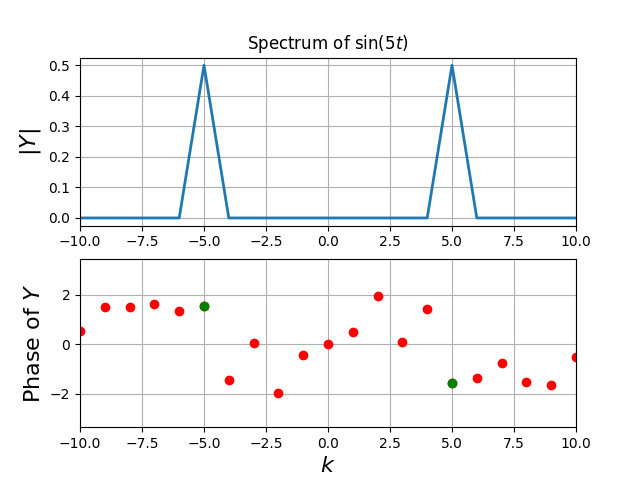
\includegraphics[scale=0.8]{Figure_2.png}
\end{figure}

\subsubsection{Spectrum of \textbf{$(1+0.1\cos(t))\cos(10t)$}}

\begin{equation*}
    f(t) = (1 + 0.1\cos(t))\cos(10t)
\end{equation*}
We plot the magnitude and phase plot of this function using the following code:
\begin{lstlisting}[language = Python]
#plotting the spectrum of (1+0.1cos(t))cos(10t)
t=linspace(0,2*pi,129);t=t[:-1]
y=(1+0.1*cos(t))*cos(10*t)
Y=fftshift(fft(y))/128.0
w=linspace(-64,64,129); w = w[:-1]

subplot(2,1,1)
plot(w,abs(Y),lw=2)
xlim([-15,15])
ylabel(r"$|Y|$",size=16)
title(r"Spectrum of $\left(1+0.1\cos\left(t\right)\right)\cos\left(10t\right)$")
grid(True)
subplot(2,1,2)
plot(w,angle(Y),'ro',lw=2)
xlim([-15,15])
ylabel(r"Phase of $Y$",size=16)
xlabel(r"$\omega$",size=16)
grid(True)
show()
\end{lstlisting}

\begin{figure}[H]
    \centering
    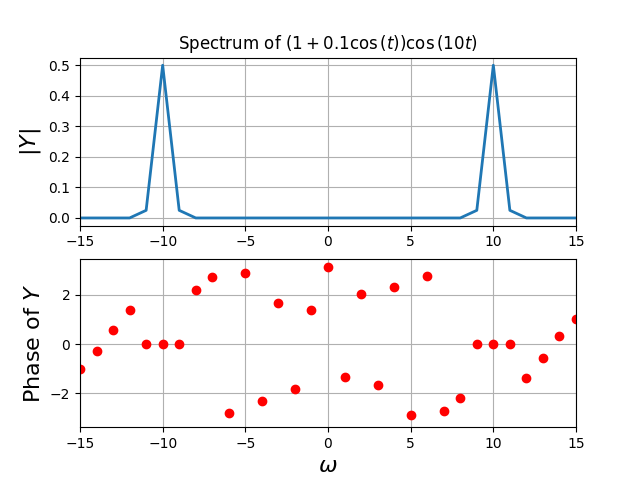
\includegraphics[scale = 0.8]{Figure_3.png}
\end{figure}

The number of sample considered is small to realize all the peaks clearly, so we plot again using more number of sample points. This is done as follows:

\begin{lstlisting}[language = Python]
#plotting the spectrum of (1+0.1cos(t))cos(10t) shifted, with higher sampling rate
t=linspace(-4*pi,4*pi,513);t=t[:-1]
y=(1+0.1*cos(t))*cos(10*t)
Y=fftshift(fft(y))/512.0
w=linspace(-64,64,513);w=w[:-1]

subplot(2,1,1)
plot(w,abs(Y),lw=2)
xlim([-15,15])
ylabel(r"$|Y|$",size=16)
title(r"Spectrum of $\left(1+0.1\cos\left(t\right)\right)\cos\left(10t\right)$")
grid(True)
subplot(2,1,2)
plot(w,angle(Y),'ro',lw=2)
xlim([-15,15])
ylabel(r"Phase of $Y$",size=16)
xlabel(r"$\omega$",size=16)
grid(True)
show()
\end{lstlisting}
The following plot is now obtained:

\begin{figure}[H]
    \centering
    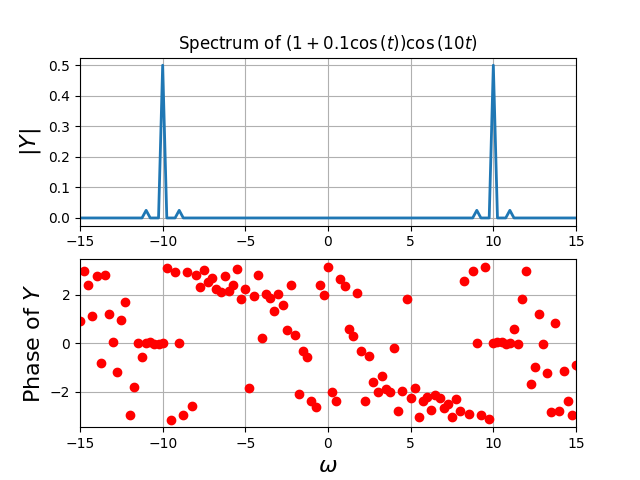
\includegraphics[scale = 0.8]{Figure_4.png}
\end{figure}

\subsection{Question 2}
\subsubsection{Spectrum of $\sin^3(t)$}
We can write $\sin^3(t)$ as:
\begin{equation*}
    \sin^3(t) = \frac{3}{4}\sin(t) - \frac{1}{4}\sin(3t)
\end{equation*}
So we should get 4 peaks at $\pm$1 and $\pm$3 with phase being $\pm\frac{\pi}{2}$.

The code is as follows:
\begin{lstlisting}[language = Python]
#plotting the spectrum of sin^3(t)
t=linspace(-4*pi,4*pi,513);t=t[:-1]
y=sin(t)**3
Y=fftshift(fft(y))/512.0
w=linspace(-64,64,513);w=w[:-1]


subplot(2,1,1)
plot(w,abs(Y),lw=2)
xlim([-15,15])
ylabel(r"$|Y|$",size=16)
title(r"Spectrum of (sin(t))^3")
grid(True)

subplot(2,1,2)
ii = where(abs(Y)>1e-3)
plot(w[ii],angle(Y[ii]),'ro',lw=2)
xlim([-15,15])
ylabel(r"Phase of $Y$",size=16)
xlabel(r"$\omega$",size=16)
grid(True)

show()
\end{lstlisting}

\begin{figure}[H]
    \centering
    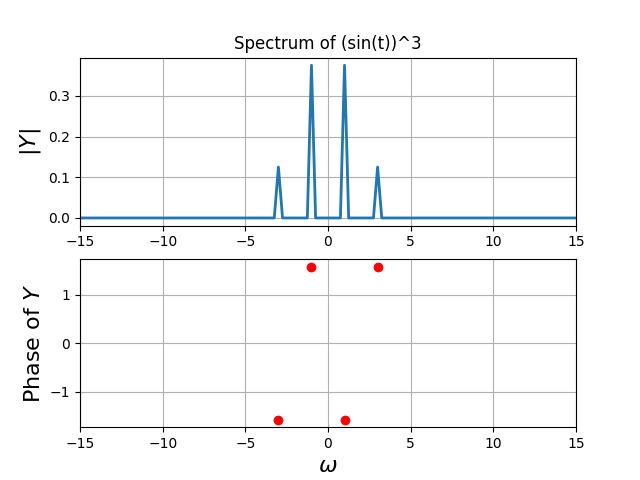
\includegraphics[scale = 0.8]{Figure_5.png}
\end{figure}

\subsubsection{Spectrum of $\cos^3(t)$}
We can write $\cos^3(t)$ as:
\begin{equation*}
    \cos^3(t) = \frac{3}{4}\cos(t) + \frac{1}{4}\cos(3t)
\end{equation*}
So we should get 4 peaks at $\pm$1 and $\pm$3 with phase being 0 or $\pi$

The code is as follows:
\begin{lstlisting}[language = Python]
#plotting the spectrum of cos^3(t)
t=linspace(-4*pi,4*pi,513);t=t[:-1]
y=cos(t)**3
Y=fftshift(fft(y))/512.0
w=linspace(-64,64,513);w=w[:-1]


subplot(2,1,1)
plot(w,abs(Y),lw=2)
xlim([-15,15])
ylabel(r"$|Y|$",size=16)
title(r"Spectrum of (cos(t))^3")
grid(True)

subplot(2,1,2)
ii = where(abs(Y)>1e-3)
plot(w[ii],angle(Y[ii]),'ro',lw=2)
xlim([-15,15])
ylabel(r"Phase of $Y$",size=16)
xlabel(r"$\omega$",size=16)
grid(True)

show()
\end{lstlisting}

\begin{figure}[H]
    \centering
    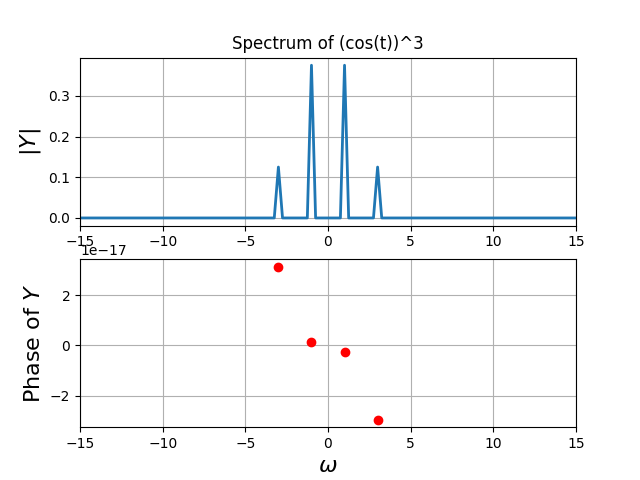
\includegraphics[scale = 0.8]{Figure_6.png}
\end{figure}

\subsection{Question 3}
We find the spectrum of the following function:
\[f(t) = \cos(20t + 5\cos(t))\]

\begin{lstlisting}[language = Python]
#plotting the spectrum of cos(20*t+5cos(t))
t=linspace(-4*pi,4*pi,513);t=t[:-1]
y=cos(20*t+5*cos(t))
Y=fftshift(fft(y))/512.0
w=linspace(-64,64,513);w=w[:-1]


subplot(2,1,1)
plot(w,abs(Y),lw=2)
xlim([-30,30])
ylabel(r"$|Y|$",size=16)
title(r"Spectrum of (cos(20*t+5cos(t)))")
grid(True)

subplot(2,1,2)
ii = where(abs(Y)>1e-3)
plot(w[ii],angle(Y[ii]),'ro',lw=2)
xlim([-30,30])
ylabel(r"Phase of $Y$",size=16)
xlabel(r"$\omega$",size=16)
grid(True)

show()
\end{lstlisting}

\begin{figure}[H]
    \centering
    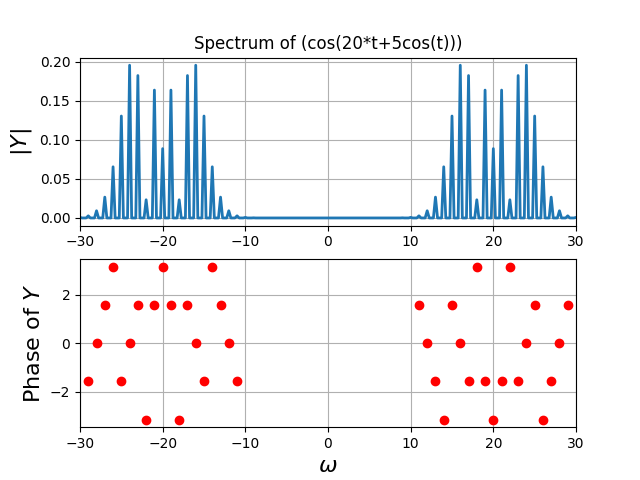
\includegraphics[scale = 0.8]{Figure_7.png}
\end{figure}

It is obvious from the plots that no longer a single peak carries all the energy and that the energy is distributed between many peaks hence the signal can be used as the dirac response of a signal modulator.

\subsection{Question 4}
The Fourier Transform of a signal is defined as:
\begin{equation*}
    X(\omega) = \frac{1}{2\pi} \int_{-\infty}^{\infty} x(t) e^{-j\omega t} dt
\end{equation*}

We can approximate the Gaussian using a sufficiently large window as the Gaussian tends to zero for large values of x, so we can approximate the integral for a window size of T(Let) as:
\begin{equation*}
    X(\omega) = \frac{1}{2\pi} \int_{-T/2}^{T/2} x(t) e^{-j\omega t} dt
\end{equation*}
Writing the integral as a Riemann summation of $N$ terms, we get:
\begin{equation*}
    X(\omega) \approx \frac{T}{2\pi N} \sum_{n = -N/2}^{N/2 - 1} x(nT/N) e^{-j\omega nT / N}
\end{equation*}
Where $T / N$ is the time step. Then, let $\omega = 2\pi k / T$:
\begin{equation*}
    X(2\pi k / T) \approx \frac{T}{2\pi N} \sum_{n = -N/2}^{N/2 - 1} x(nT/N) e^{-j2\pi kn/N}
\end{equation*}
We see that the summation is the DFT(Discrete Fourier Transform) of the signal. Thus, we get:
\begin{equation*}
    X(2\pi k / T) \approx \frac{T}{2\pi N} DFT\{x(nT/N)\}
\end{equation*}
We can improve the accuracy of our obtained approximation by choosing a larger window size while keeping the sampling frequency constant, this is done by doubling both the range and the number of samples, thus the sampling frequency remains constant. We do this iteratively until our error is below a certain threshold.\\

We compare our approximation to the actual CTFT(Continuous Time Fourier Transform) of the Gaussian:
\begin{equation*}
    F(e^{-\frac{t^2}{2}}) = \frac{1}{\sqrt{2\pi}}e^{-\frac{\omega^2}{2}}
\end{equation*}

This is done as follows:
\begin{lstlisting}[language = Python]
#Approximated spectrum of e^-t^2/2
tolerance = 1e-6
Y_old = 0
error = tolerance + 1
start = 4*pi
samples = 256
niter = 0
while error > tolerance:
    t = linspace(-start,start,samples+1);t=t[:-1]
    y = exp(-t**2/2)
    Y_approx = fftshift(fft(ifftshift(y))) * (start/(pi*samples))
    w = linspace(-samples*pi/(start*2), samples*pi/(start*2), samples+1); w=w[:-1]
    error = sum(abs(Y_approx[::2] - Y_old))
    Y_old = Y_approx
    samples = samples*2
    start = start*2
    niter = niter + 1

#plotting approximated spectrum


subplot(2,1,1)
plot(w,abs(Y_approx),lw=2)
xlim([-15,15])
ylabel(r"$|Y|$",size=16)
title(r"Approximate Spectrum of e^-t^2/2")
grid(True)

subplot(2,1,2)
phi = angle(Y_approx)
phi[where(abs(Y_approx)<1e-3)] = 0
plot(w,phi,'ro',lw=2)
xlim([-15,15])
ylabel(r"Phase of $Y$",size=16)
xlabel(r"$\omega$",size=16)
grid(True)
show()
\end{lstlisting}

\begin{figure}[H]
    \centering
    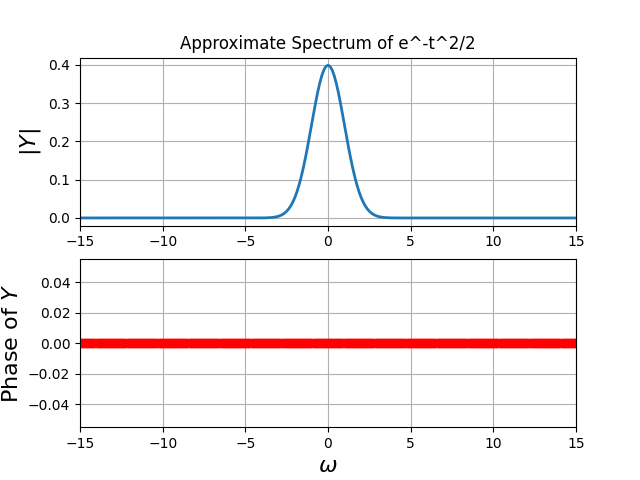
\includegraphics[scale = 0.7]{Figure_8.png}
\end{figure}

\begin{lstlisting}[language = Python]
#True Spectrum
#t and w are same as above
y = exp(-t**2/2)
Y_true =  1/sqrt(2*pi)*exp(-w**2/2)#fourier transform of a gaussian function is a gaussian function

subplot(2,1,1)
plot(w,abs(Y_true),lw=2)
xlim([-15,15])
ylabel(r"$|Y|$",size=16)
title(r"True Spectrum of e^-t^2/2")
grid(True)

subplot(2,1,2)
plot(w,angle(Y_true),'ro',lw=2)
xlim([-15,15])
ylabel(r"Phase of $Y$",size=16)
xlabel(r"$\omega$",size=16)
grid(True)

show()

\end{lstlisting}

\begin{figure}[H]
    \centering
    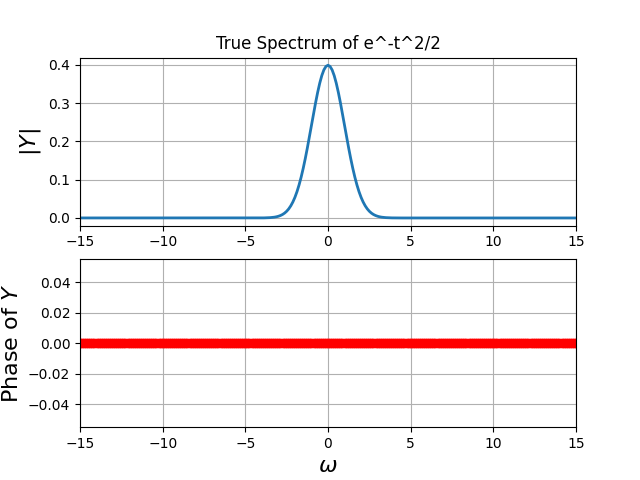
\includegraphics[scale = 0.8]{Figure_9.png}
\end{figure}

Comparing the two spectrums on the same graph:
\begin{lstlisting}[language = Python]
#Plotting the two spectrums on the same graph:
plot(w,abs(Y_true),lw=2)
plot(w,abs(Y_approx), 'r--', lw=2)
xlim([-15,15])
ylabel(r"$|Y|$",size=16)
title(r"True and Approximate Spectrum of e^-t^2/2")
grid(True)
legend(["True Spectrum","Approximate Spectrum"])
show()

true_error = sum(abs(Y_approx - 1/sqrt(2*pi)*exp(-w**2/2)))
print("Error: " + str(true_error))
\end{lstlisting}
The error comes out to be \\
Error: 1.86620529933118e-14
Thus, we see that our approximation is very accurate.

\begin{figure}[H]
    \centering
    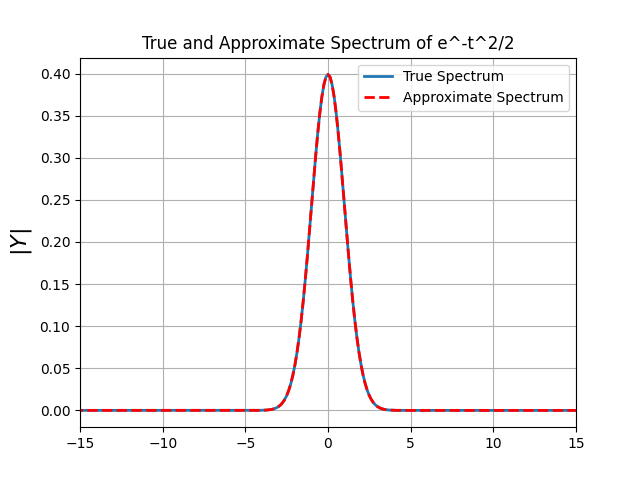
\includegraphics[scale = 0.8]{Figure_10.png}
\end{figure}

 \section{Conclusion}
We explored the \texttt{numpy.fft} module by using it to find the Fourier and Inverse Fourier Transforms of various signals. We learnt about the DFT and implementing it using FFT. We also learnt to approximate the CTFT of a function using an iterative approach.

\end{document}




 